\chapter{Results}
\label{chap:res}
\section*{Chapter Outline}
In this chapter we present the results generated from the various experiments. We first present the results of the link-level delay estimation using cross-correlation and show the analysis of the performance of this estimator. We then present the results of the investigation of the mutual information between two cells, and show how there is little to no correlation between the link-parameters and the calculated results. Finally, we present the results of the cell-classification model, and compare the performance of the various classifiers.


\section{Neuronal-Link Parameters}
% \begin{itemize}
%     \item Some graphs of the stimulus/response spike-trains
%     \item Some graphs on the discretisation of a spike train into a binary sequence.
%     \item Some plots of the estimated mutual information vs network parameters
%     \item R-scores of the correlation between the mutual information and the parameters
% \end{itemize}
% TODO: bad results cos not enough data? Cite da paper.

\subsection{Delay Estimation}
As stated in \ref{chap:meth:llMeth}, the analysis of the link-level details of a synaptic connected was done through the simulation of around 10,000 simple 2-cell networks. This results in the production of sets of voltage data for each simulation, one from the "head" cell and one from the "tail" cell. As the output of one cell is acting as the stimulus to the other, the spike trains from the simulations tend to be correlated. The output plots of a number of a few of these simulations is shown in Figure \ref{fig:sample2CellPlots}. In these sample plots, the source-destination spike correlation is clear to see as a spike in the pre-synaptic cell often results in a spike in the post-synaptic cell. As well as this, the plots indicate a slight delay between the source and event spikes.
\begin{figure}[ht]
    \centering
    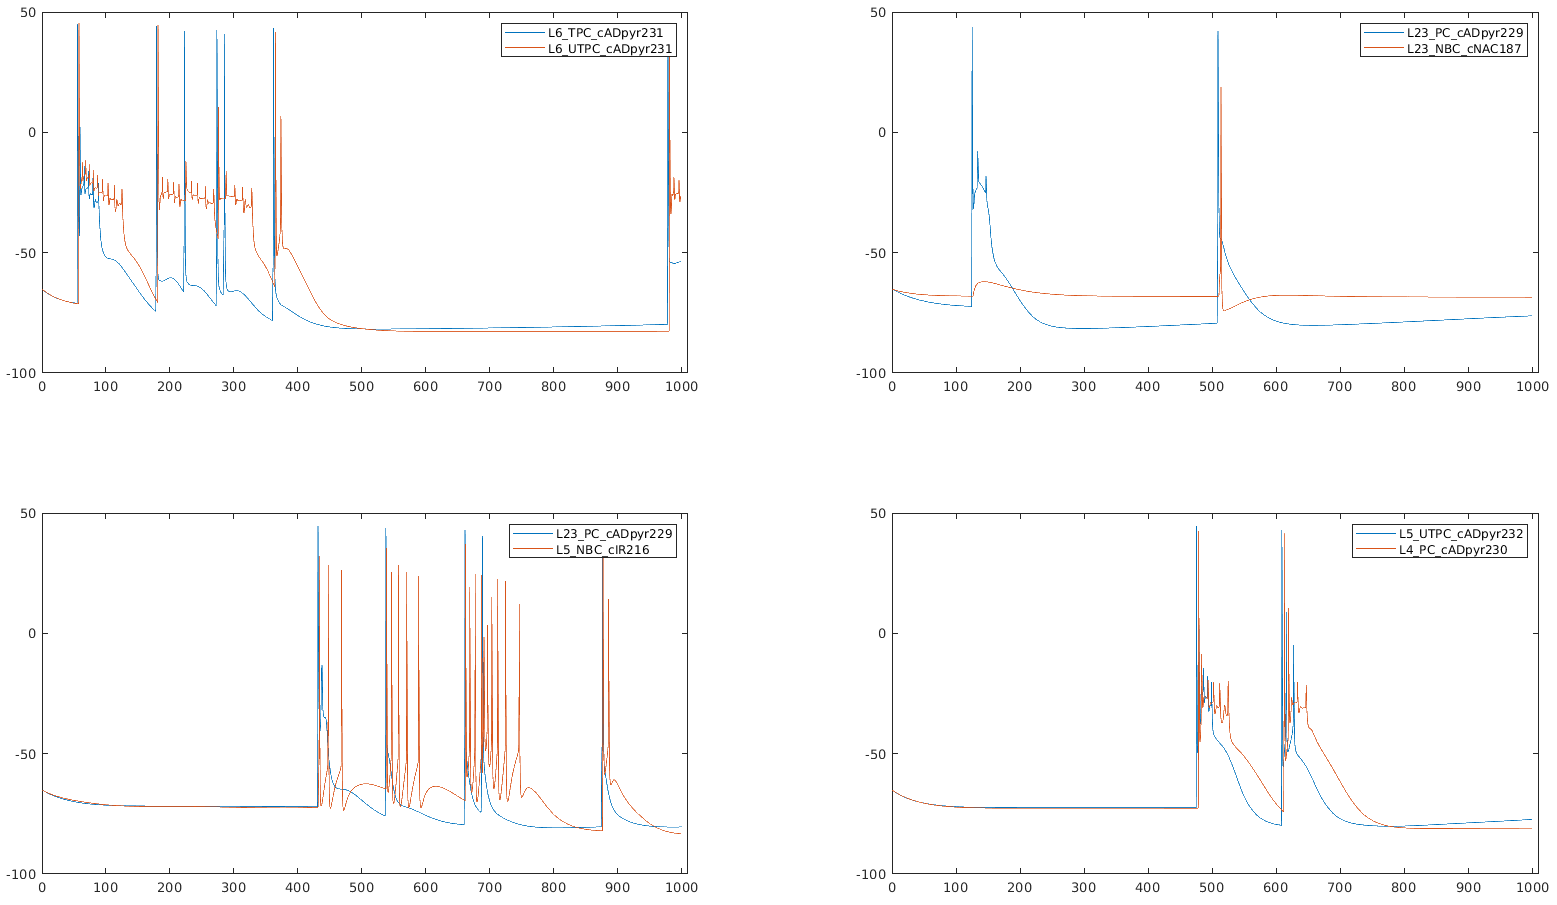
\includegraphics[width=\textwidth]{05-Results/2cellComp.png}
    \caption{Comparison of 2-cell network outputs. Head cell in blue, tail cell in orange. Cell-types shown in each subplot's legend}
    \label{fig:sample2CellPlots}
\end{figure}

\par

Following the collection of the simulation data, analysis was done on the estimation of the link delay through the use of the cross-correlation between the two measured voltage plots. This was implemented by loading the two cell voltage series, and using the Matlab \emph{xcorr()} function to get the cross-correlation of the two series to a specified number of lags. Next, we find the closest positive peak in the cross-correlation using the \emph{findpeaks()} function. This function finds the local maxima in a series which are the portions of the plot where the first derivative is 0 and the second derivative is negative (concave-down). By making the assumption that the first local maxima represents the delay, we can obtain a simple estimate of the link delay. Figure \ref{fig:sample2CellCorrPlots} shows a number of plots representing this delay estimation. Each subplot shows the cross-correlation of the 2 signals at a number of lag values from -12ms to +12ms, along with the location of the estimated link delay (i.e. the location of the first positive peak) and the location of the actual link delay (as specified by the \emph{delay} parameter in the associated \emph{NetCon} object.\\

\begin{figure}[ht]
    \centering
    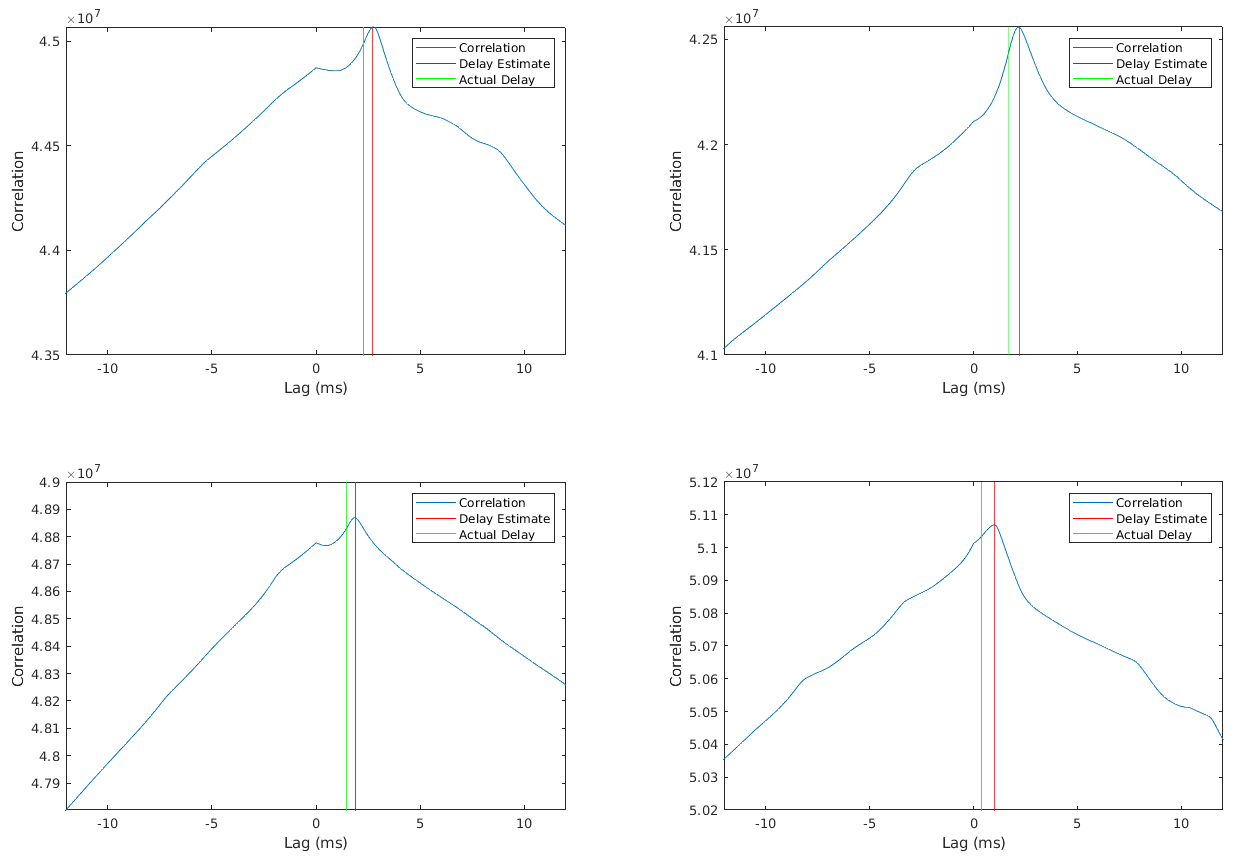
\includegraphics[width=\textwidth]{05-Results/2cell_Corr.png}
    \caption{Comparison of 2-cell cross-correlation with delay estimate. Cross-correlation shown in blue, estimated delay as a vertical red line, actual delay as a vertical green line}
    \label{fig:sample2CellCorrPlots}
\end{figure}

With this method of delay estimation, the estimator was run against all the simulated networks (N=10,000) and the correlation between the estimated delay and the actual delay was analysed. First, the estimations of 0ms were removed, as this was the "error value" returned by the estimator when it was unable to determine the actual delay (possibly due to a lack of spike-data in the simulation). A linear model was then fit to the data in order to determine the correlation between the estimation and the actual delay. A scatter-plot of the estimation and actual delay is shown in \ref{fig:2CellDelayLFit} along with the least-squares linear fit and associated R-squared score. The mean-squared error of this linear model was 1.0881.
\begin{figure}[ht]
    \centering
    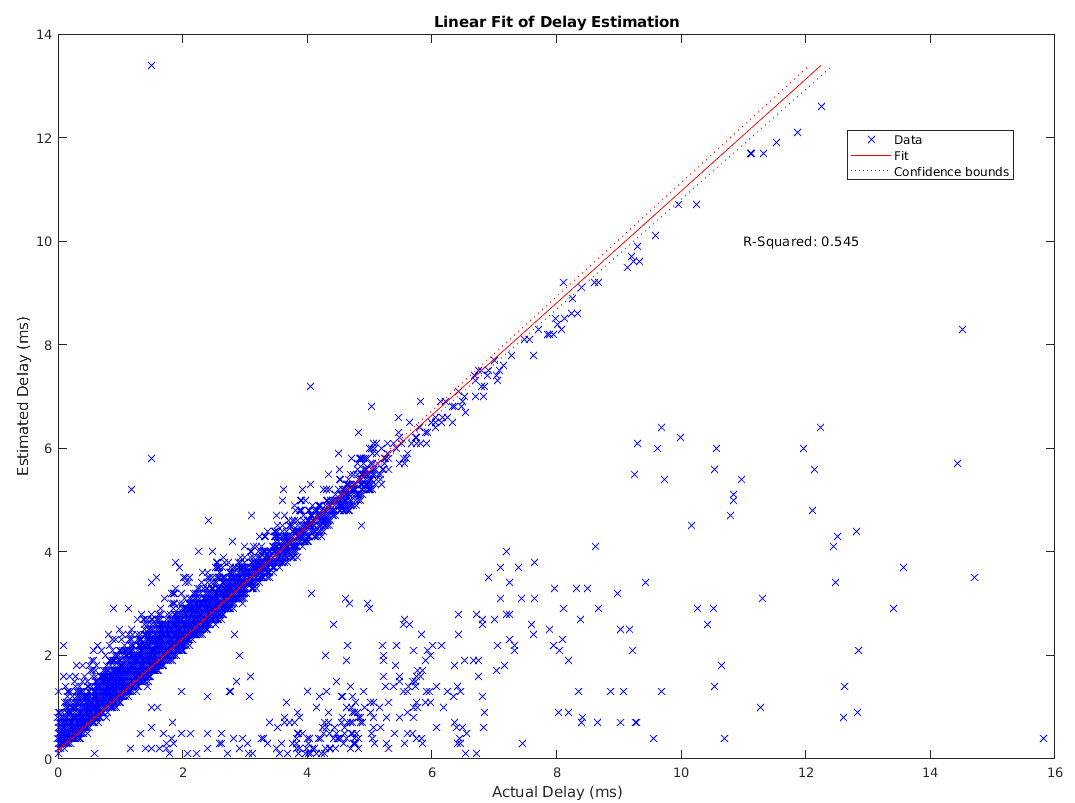
\includegraphics[width=0.8\textwidth]{05-Results/delayFit.png}
    \caption{Correlation of delay estimate vs actual delay with least-squares linear model and associated R-squared score}
    \label{fig:2CellDelayLFit}
\end{figure}

\subsection{Entropy and Mutual Information}
As discussed in \ref{chap:meth:llMeth}, the entropy of the cells is calculated by discretising the spike train and treating it as though the spikes represent a single binary symbol. The process for this is outlined in \ref{fig:discrTrain} and was again implemented in Matlab. Using the symbol sequence it is then possible to apply the corresponding equations (\ref{eq:entropyDiscr}, \ref{eq:mutualInf}) to determine the entropy of the individual cells, and the mutual information of the cell-to-cell connection. As well as this, we can use the delay estimation model described above, which allows us to shift the spike train of the "tail" cell such that the spike-response should be instantaneous. This is done to investigate whether or not adjusting for the delay in the link will effect the calculated mutual information.\\
The probability-mass function (PMF) of the calculated single-cell entropy is shown in Figure \ref{fig:cellEntPmf}. The majority of the cells have an entropy of below 0.4 bits/symbol, with a continuously decreasing proportion of the cells having an increasing entropy. The PMF of the calculated mutual information is shown in Figure \ref{fig:mutualInfoPmf}. We can see that the mutual information of the networks is well-distributed, with a mean of around 0.5 bits. Of note here is that the effect of shifting the spike-train based on the delay estimate has little to no effect on the distribution of the mutual information. \\

\begin{figure}

\centering
\begin{subfigure}[b]{0.9\textwidth}
    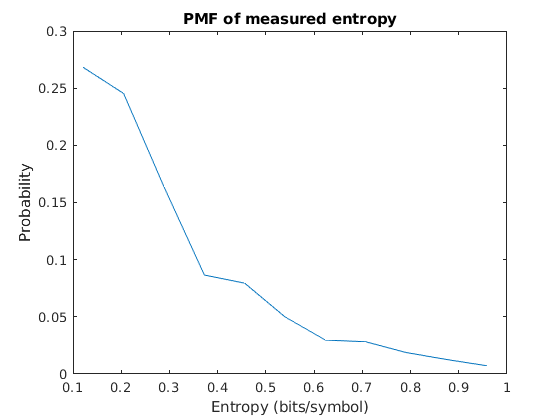
\includegraphics[width=1.0\textwidth]{05-Results/entropyPmf.png}
    \caption{PMF of calculated single-cell entropy based on output spike trains}
    \label{fig:cellEntPmf}
\end{subfigure}

\begin{subfigure}[b]{0.9\textwidth}
    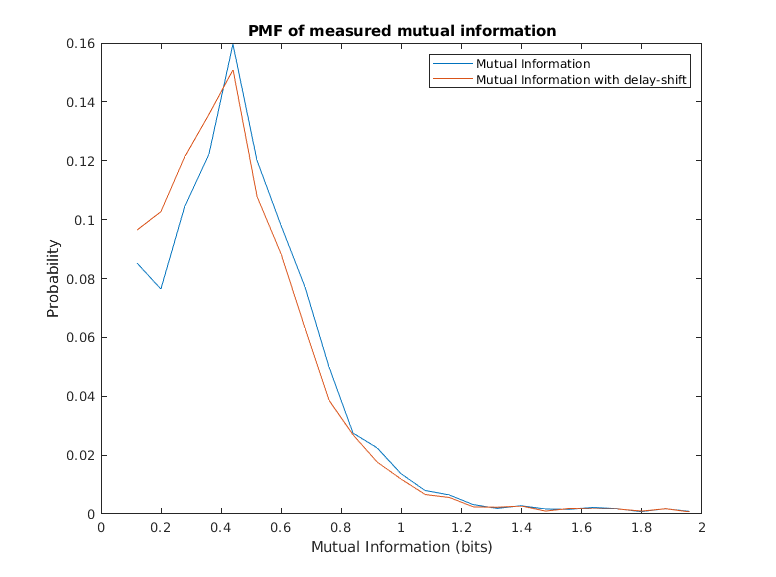
\includegraphics[width=1.0\textwidth]{05-Results/mutualInfo_pmf.png}
    \caption{PMF plots of calculated mutual information for the measured spike-train (blue) and the delay-estimate shifted spike-train (orange)}
    \label{fig:mutualInfoPmf}
\end{subfigure}
\caption{PMF of 2-cell entropy and mutual information}
\end{figure}


% \begin{figure}[ht]
%     \centering
%     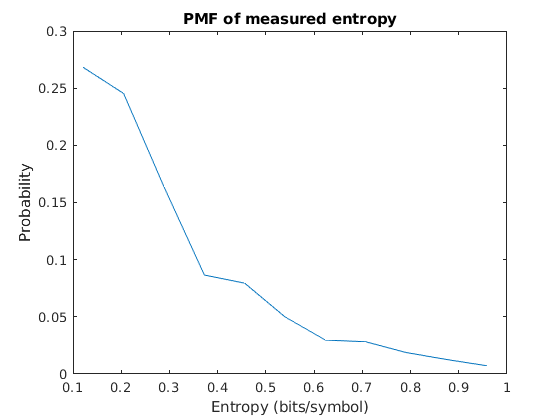
\includegraphics[width=0.9\textwidth]{05-Results/entropyPmf.png}
%     \caption{PMF of calculated single-cell entropy based on output spike trains}
%     \label{fig:cellEntPmf}
% \end{figure}

% \begin{figure}[ht]
%     \centering
%     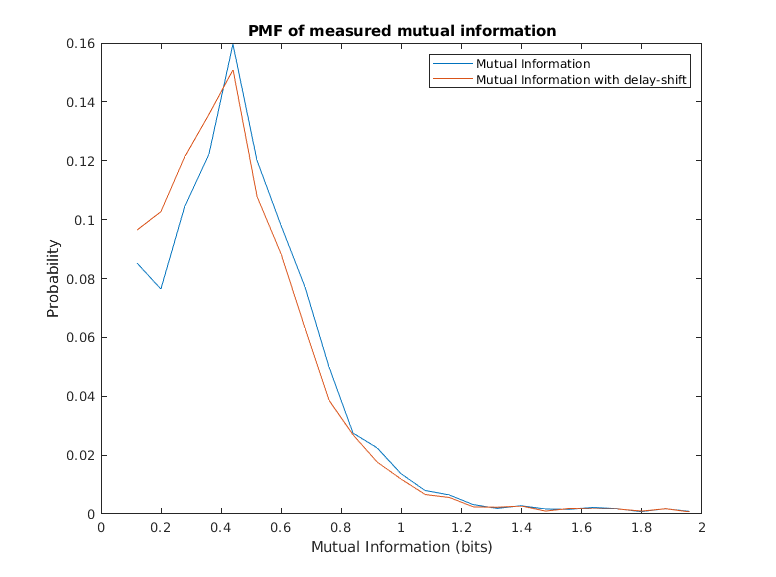
\includegraphics[width=0.9\textwidth]{05-Results/mutualInfo_pmf.png}
%     \caption{PMF plots of calculated mutual information for the measured spike-train (blue) and the delay-estimate shifted spike-train (orange)}
%     \label{fig:mutualInfoPmf}
% \end{figure}

We next look at the possible factors that may have an effect on the mutual information. We can plot a number of scatter-graphs to visually represent any correlations in the data, as shown in Figure \ref{fig:mInfoCorrGraph}. In this figure, we can examine any correlation between the mutual information and the number of synapses in the connection, the delay in ms of the link, the weight of the link, and the distance between the 2 cells in the network. We can see that there is no obvious correlation between any of the link-level parameters and the mutual information of the network.\\
\begin{figure}[ht]
    %\centering
    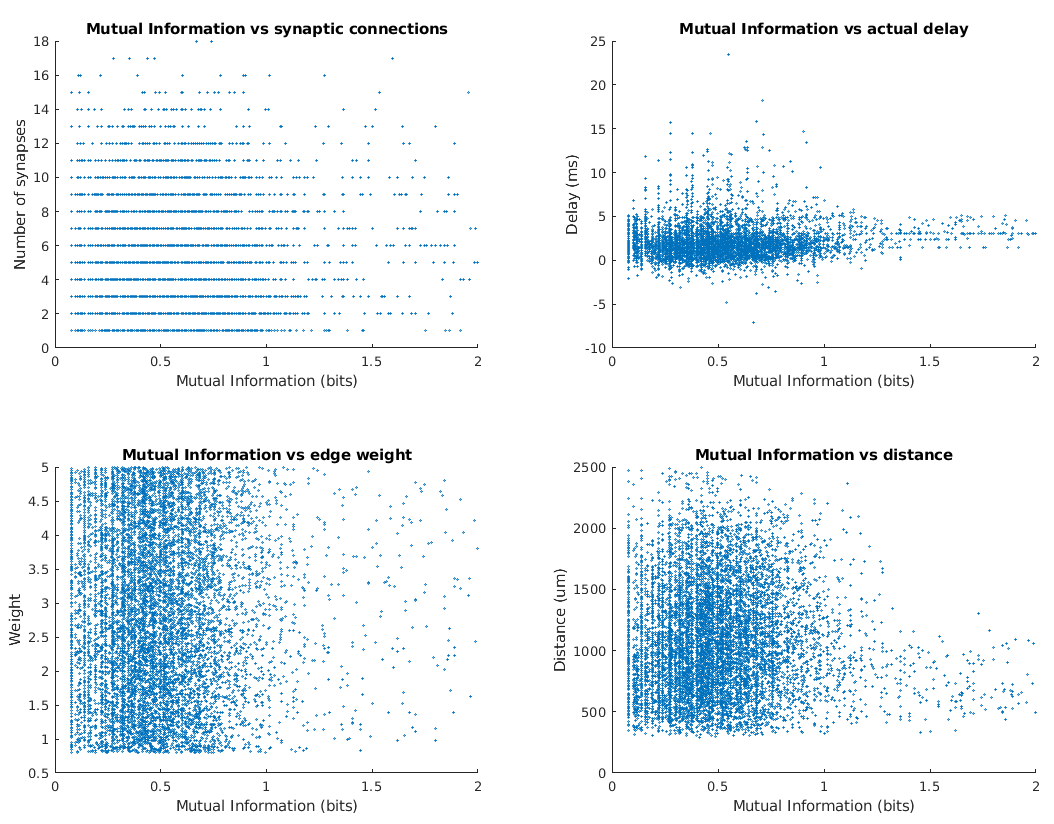
\includegraphics[width=\textwidth]{05-Results/minfoCorrPlot.png}
    \caption{Scatter plots of measured mutual information vs number of synapses, edge delay, edge weight, and distance between the cells.}
    \label{fig:mInfoCorrGraph}
\end{figure}
While there is no obvious correlation between any single parameter and the mutual information, these 2-d plots do not take into account all of the link parameters at once; that is, it could be that correlation could be found by analysing the dimension-space made up of all measured parameters. This can be done using a linear model, as used to determine the correlation in the delay estimate. In this case, we use multiple predictor variables (the link parameters) and a single response variable (the mutual information). This model is shown in Figure \ref{fig:lmInfo}. With an R-squared score of 0.034, it is clear that there is no correlation between the network parameters and the mutual information of the neural link.
\begin{figure}[ht]
    \centering
    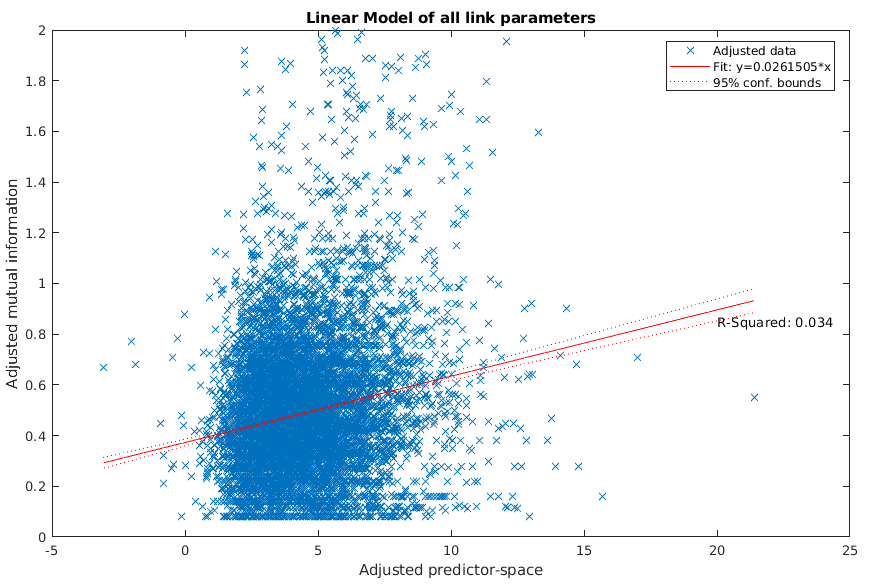
\includegraphics[width=\textwidth]{05-Results/lmMinfo.png}
    \caption{Linear fit of all network parameters to predict mutual information}
    \label{fig:lmInfo}
\end{figure}


\section{Classification}

\subsection{2-Cell Classification and Model Training}
% \begin{itemize}
%     \item Spike train figures showing the difference in impulse response between cells
%     \item Some figures of the LNP estimation and associated coefficients
%     \item Some scores on the separation of the filter coefficients between cell classes
%     \item Confusion matrices and different model metrics for the classification models, and the differences in the analysed algorithms (GMM, SVM, NN etc)
% \end{itemize}
% TODO: above

In Figure \ref{fig:sample2CellPlots} a number of spike-trains from different cell types were shown. Referring back to this, it is clear that different cells respond different to stimulus, with the output spike train differing in intensity (frequency of spikes) as well as in the "settle-down" period after a spike was triggered (i.e. the fall-time response of the membrane voltage). It is these differences that we attempt to characterise through the use of the linear-filter portion of the linear-nonlinear-Poisson (LNP) cascade model.\\
The first step in this process is to simulate a number of 2-cell networks again in order to generate test data. In this instance, the "head" cell acts only as a stimulus generator, and we treat the soma-membrane potential of this cell as the "input" voltage to the linear system described in \ref{eq:firLinSys}. In order to limit the number of variables in this investigation, the type of cell used as the head cell was constant across all simulations (layer 1, DAC m-type, bNAC e-type) while the "tail" cell was treated as the cell-under-test and so was varied between simulations. As well as this, variations in link-level parameters (number of synapses etc.) were kept to a minimum to reduce the number of variables. A large number of networks were generated (N=30,000) in order to produce a dataset of sufficient size for classifier training.
Following simulation and prior to training the classifiers, the filter estimation step described in equation \ref{eq:estFilter} was applied to extract the filter coefficients as features from the cell-response data. Figure \ref{fig:sampImpRes} shows the filter coefficients (FIR impulse response) of 4 different cells, with a filter-order of 64. It is clear from this diagram that the impulse-response estimation of the neuronal cell is capable of differentiating between the cell types. Using these estimated filter coefficients, we are now able to begin training the classifiers.
\begin{figure}[ht]
    \centering
    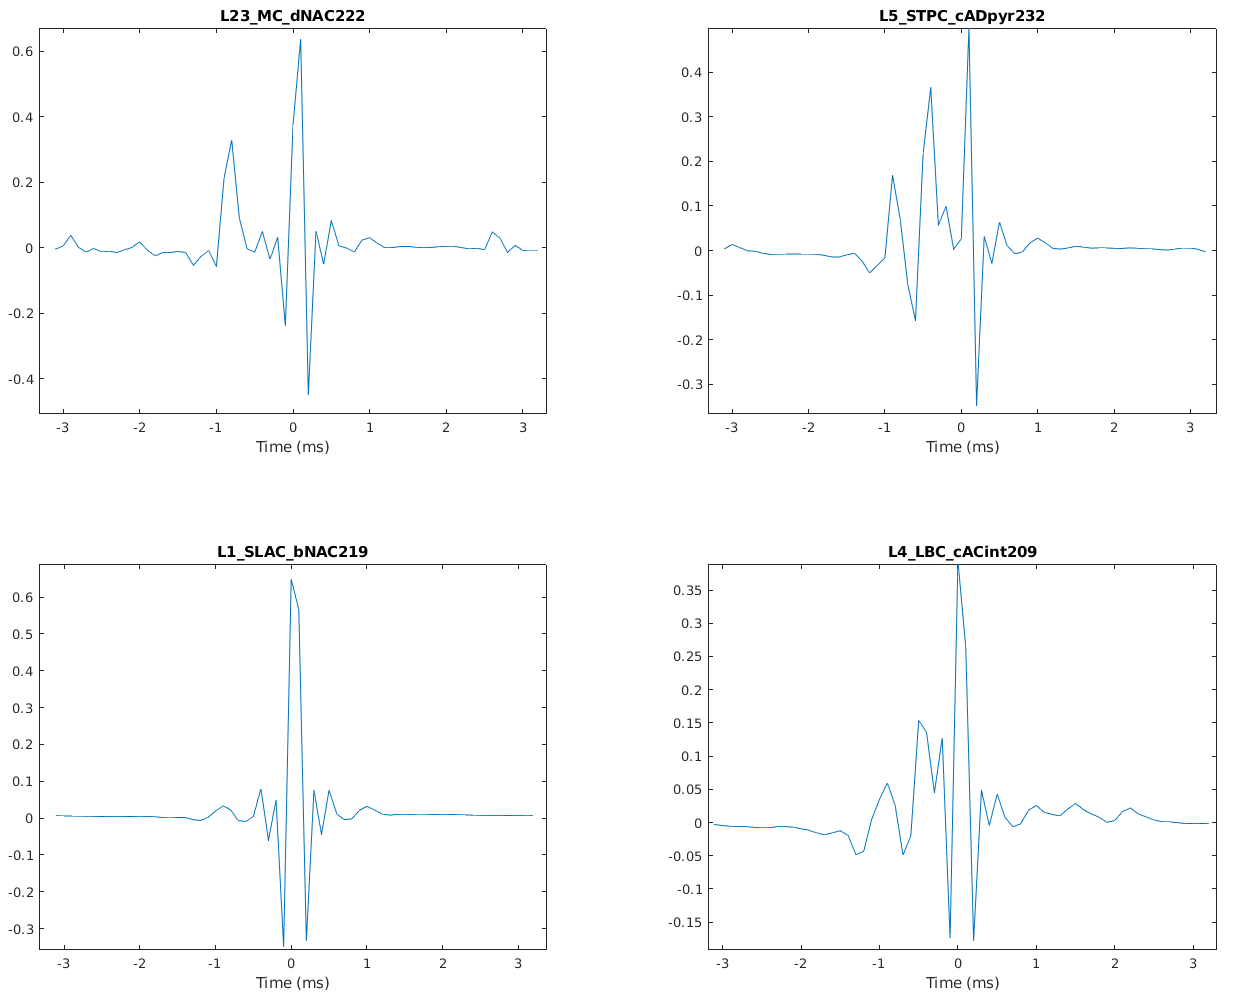
\includegraphics[width=\textwidth]{05-Results/sampImpRes.png}
    \caption{Sample impulse-response characterisation of different cells}
    \label{fig:sampImpRes}
\end{figure}

\par

Using the previously discussed \emph{Classification Learner} tool in Matlab, we can quickly train and compare a set of different classifiers, inspecting the accuracy, confusion matrix, and receiver-operating characteristic (ROC) curve for each. The first classifier to investigate is the layer classifier, which takes the estimated filter coefficients as input, and attempts to estimate what layer the characterised cell belongs to. Of the classifiers discussed in \ref{chap:back:class}, we can train and analyse SVM and Decision Tree classifiers. Using RapidMiner, we can also train artificial neural networks (NN), and the Random-Forest variation of the Decision Tree classifier.\\
The performance of the classifiers are shown in the following tables. In each table, we compare the performance of the different classification algorithms (Decision Tree, SVM etc.) in the classification of the separate cell sub-group types (layer, m-type, e-type). For each classifier we state the corresponding accuracy. The accuracy is calculated as the ratio of correct estimations versus incorrect estimations. We also state the "factor improvement" of the classifier. This is calculated as the factor by which the classifier improves over the equivalent accuracy of random guessing in the classification space. For example, with 5 layer classes the equivalent "random guess" accuracy is 20\%, and so a trained classifier with accuracy of 40\% would have a factor improvement of 2. \\

Table \ref{tbl:layerClassifierPerf} shows the performance of the classifiers in the prediction of cell layer-type, table \ref{tbl:mtypeClassifierPerf} for m-type prediction, and table \ref{tbl:etypeClassifierPerf} for e-type prediction. In every case, the SVM classifier has the highest accuracy, with the NN being slightly behind. Of the tree-based classifiers, interestingly the decision tree based classifier has a consistently higher accuracy than the random forest classifier, despite the latter being a variant of the former. 


\begin{table}[h]
    \centering
    \begin{tabular}{|c||c|c|c|c|}
        \hline
        Classifier & Decision Tree & Random Forest & SVM & NN\\
        \hline\hline
        Accuracy & 52.2\% & 41.43\% & 62.5\% & 60.98\%\\
        \hline
        Factor Improvement & 2.61 & 2.07 & 3.13 & 3.05 \\
        \hline
    \end{tabular}
    \caption{Performance of different algorithms at classifying cell-layer (5 classes, 20\% equivalent random guessing accuracy)}
    \label{tbl:layerClassifierPerf}
\end{table}

\begin{table}[h]
    \centering
    \begin{tabular}{|c||c|c|c|c|}
        \hline
        Classifier & Decision Tree & Random Forest & SVM & NN\\
        \hline\hline
        Accuracy & 42.6\% & 35.07\% & 63.7\% &57.99\%\\
        \hline
        Factor Improvement & 10.65 & 8.77 & 15.93 &13.92\\
        \hline
    \end{tabular}
    \caption{Performance of different algorithms at classifying cell m-type (25 classes, 4\% equivalent random guessing accuracy)}
    \label{tbl:mtypeClassifierPerf}
\end{table}

\begin{table}[h]
    \centering
    \begin{tabular}{|c||c|c|c|c|}
        \hline
        Classifier & Decision Tree & Random Forest & SVM & NN\\
        \hline\hline
        Accuracy & 63.8\% & 54.47\% & 75.3\% &73.94\%\\
        \hline
        Factor Improvement & 8.93 & 7.63 & 10.54 &10.35\\
        \hline
    \end{tabular}
    \caption{Performance of different algorithms at classifying cell e-type (14 classes, 7.143\% equivalent random guessing accuracy)}
    \label{tbl:etypeClassifierPerf}
\end{table}

\par

Another set of results that are often used to quantify the performance of a classifier is the class precision and the class recall. The class recall is calculated per-class as the ratio of correct predictions of a class versus the number of observations of that class. The class precision is again calculated per-class as the ratio of correct predictions of a class versus the overall number of the classifier estimated that class.  As these metrics identify the performance of the model on a class-by-class basis, it results in a large number of individual values to compare. When we consider that we are comparing 3 estimator groups with a relatively high number of classes per group (5 for layer estimator, 25 for m-type, and 14 for e-type), as well as the fact that each estimator group must be compared against 4 different classification algorithms, it becomes difficult to critically compare the performance of each individual class. In general, however, when analysing such metrics from single classifier, a \emph{confusion matrix} is used. The confusion matrix of the SVM-based layer estimator is shown in Figure \ref{fig:svmConfMatLayer}. The confusion matrix tabulates the estimations of a given classifier as a grid of "True Class" versus "Predicted Class". In this way, it can show how often an observation of a given class is estimated as belonging to some other class. As such, the diagonal (shown as green in the confusion matrix figure) shows the proportion of the correct predictions in the validation set (where true class equals predicted class). The right hand bar shows the proportional difference of the \emph{true positive rate} and the {false negative rate}. This true-positive rate is equivalent to the class recall.\\
While the confusion matrices for every single classifier investigated in this study are not included, the relative proportions between them tend to be similar (i.e. very high prediction accuracy between layer 1 and layer 6, with reduced accuracy in the intermediate layers).

\begin{figure}[ht]
    \centering
    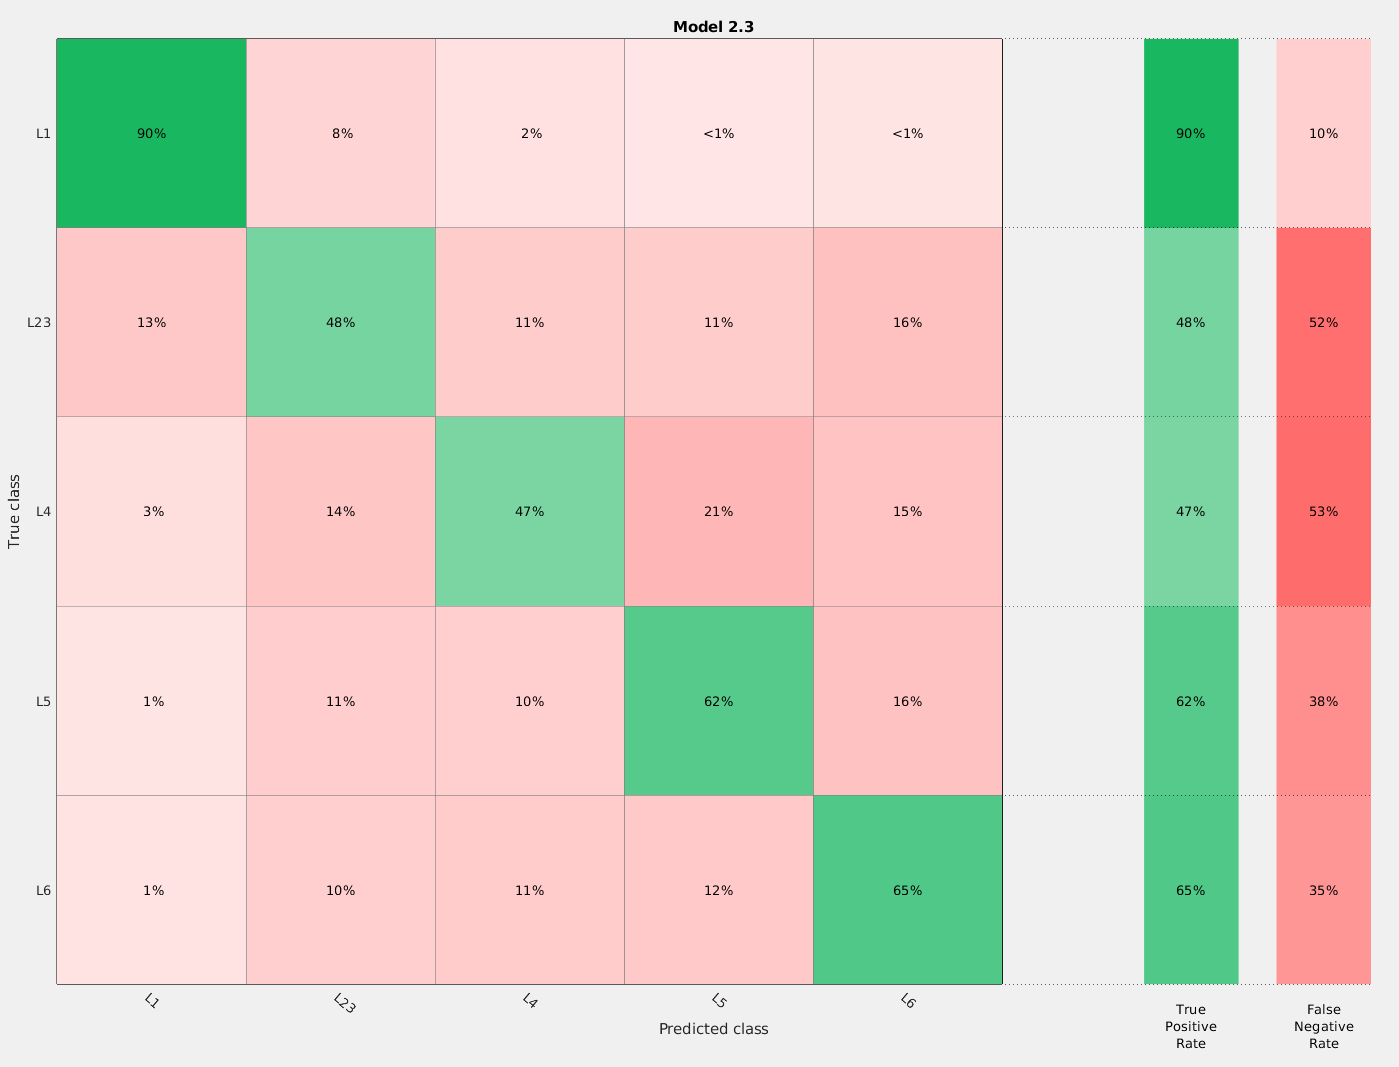
\includegraphics[width=1.0\textwidth]{05-Results/svmLayerConf.png}
    \caption{Confusion Matrix of SVM layer-classifier}
    \label{fig:svmConfMatLayer}
\end{figure}



\subsection{Network Tomography for Cellular Classification}
% \begin{itemize}
%     \item Figures of 4-leaf networks
%     \item Metrics in the reconstruction of these networks
%     \item Some figures showing the estimated network reconstruction vs actual network etc.
% \end{itemize}

As the SVM classifier had the best performance during training, this is the model that was applied in the reconstruction of the 4-leaf star networks. The process here was similar to the previous experiments: a number of unique networks were generated, simulated, and their data-points measured and analysed. In this case, the networks generated were of the 4-leaf star topology previously discussed and shown in Figure \ref{fig:4leafStar}. The central node was constrained to be of the same layer 1, DAC m-type, bNAC e-type cell type used in the training of the models, while the star cells were varied. For each measurement from the soma-membrane of a star node, the characteristic filter was estimated using the same process discussed previously, and the filter coefficients were passed through the pre-trained classifiers.

\par
The performance results of the topology reconstruction are shown in Table \ref{tbl:wholeClassifierPerf}. Here, we tabulate the accuracy of the classifier chain in estimating layer, m-type, and e-type groups, as well as the "whole-cell" classification accuracy. We define the whole-cell accuracy as the the cases where all three sub-groups were correctly estimated. Evidently, the factor-improvement for the whole-cell prediction is significantly higher than for any other group, while the sub-group accuracy is quite similar to those in the 2-cell networks.

\par

Figure \ref{fig:4CellRecon} shows a sample reconstruction of a 4-leaf network from probe measurements. The left side of the figure represents the network as it was simulated, with probes at the network endpoints and a stimulus on the central node, along with the actual cell types of the leaf nodes. The right side of the figure shows the reconstructed topology based on the cell-type estimations from the SVM classifier chain. 

\begin{figure}[ht]
    \centering
    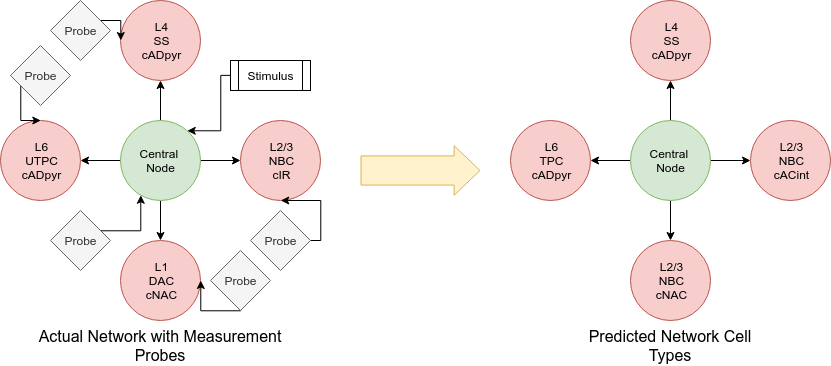
\includegraphics[width=1.0\textwidth]{05-Results/4cellTopRecon.png}
    \caption{Sample reconstruction of network}
    \label{fig:4CellRecon}
\end{figure}

\begin{table}[ht]
    \centering
    \begin{tabular}{|c||c|c|c|c|}
        \hline
        Prediction & Layer & m-type & e-type & whole-cell \\
        \hline\hline
        \# classes & 5 & 25 & 14 & 1750\\
        \hline
        Equiv. random guess accuracy & 20.0\% & 4.0\% & 7.143\% & 0.0571\%\\
        \hline
        Classifier accuracy & 61.82\% & 56.34\% & 64.62\% & 36.23\%\\
        \hline
        Factor improvement & 3.091 & 14.085 & 9.05 & 634.5\\
        \hline
    \end{tabular}
    \caption{Performance of 4-leaf star topology reconstruction}
    \label{tbl:wholeClassifierPerf}
\end{table}


